



\begin{document}\selectlanguage{ngerman}
\small
\section*{\huge{LHCb Quark-Puzzle}}
\begin{figure}[h]
    \begin{minipage}[t]{0.474\textwidth}
    %\vspace{-6.0cm}
        Das Standardmodell der Teilchenphysik haben Sie bereits im Einführungsvortrag kennengelernt. In der Abbildung rechts, sehen Sie davon die Quarks.  Nun ist es Ihre Aufgabe aus den kleinsten Bestandteilen von Materie -- den Quarks --, Teilchen zu formen. Sie erhalten im Folgenden Quarks und Antiquarks, die das Wissen der Wissenschaftler*innen beim Bau von Materie besitzen! Was hat sich die Natur dabei gedacht, wenn sie den Quarks diese Eigenschaften versieht? Welche Teilchen kann man bauen, unter welchen Bedingungen? 
    \end{minipage}~~
     \begin{minipage}[t]{0.50\textwidth}
     \centering
       \vspace{-1cm}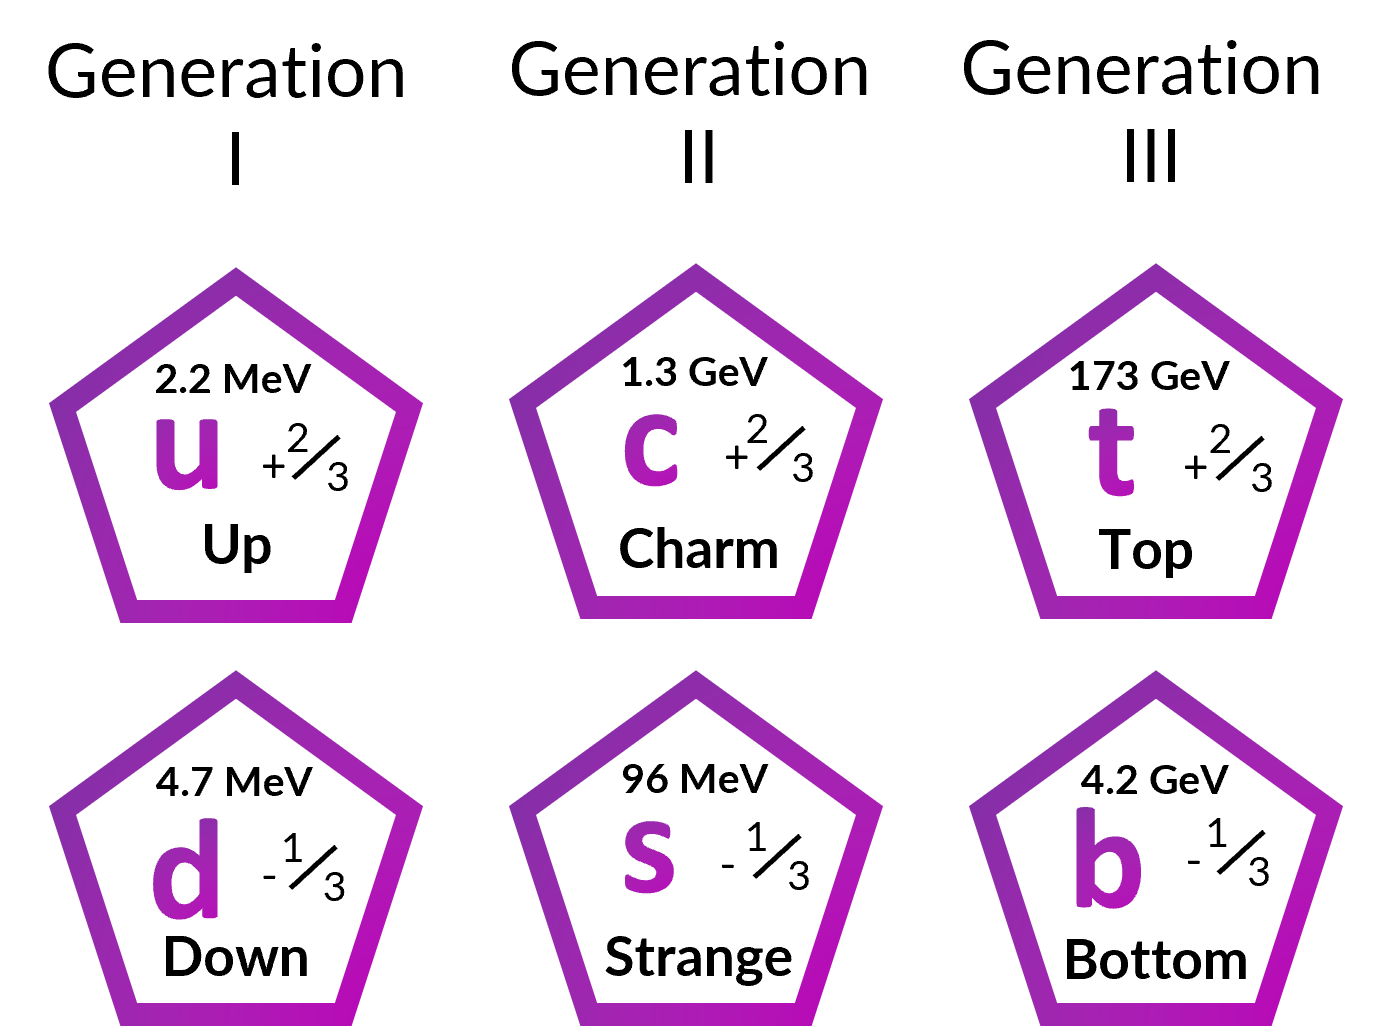
\includegraphics[width=.8\textwidth]{Figures Worksheets/Quarks_Quark_Puzzle_Worksheet.png}
         \caption{Übersicht der Quarks, ihre Massen und el. Ladungen in Einheiten von $e$. Bei Antiquarks wechselt das Vorzeichen der Ladung.}
    \end{minipage}
    \end{figure}
\SetDefinition{\textbf{Der Natur auf der Spur:} Bauen Sie aus Quarks (z.B. u) und Antiquarks (z.B. $\Bar{\textmd{u}}$) abgeschlossene Teilchen. Wie heißen Sie und unter welchen Bedienungen halten Quarks zu einem Teilchen zusammen? Gibt es Auffälligkeiten? \\  \emph{Bearbeiten Sie in Gruppenarbeit und teilen Sie Aufgaben auf:} \\ \, \\
\textbf{a)} Probieren Sie aus! Wenn Sie ein Teilchen gefunden haben, schreiben Sie die Buchstabenkombinationen der Quarks auf (das nennt man den Quarkinhalt) \\ \, \\
\textbf{b)} Wie heißen Ihre Teilchen? Rufen Sie mit Ihrem PC oder Smartphone die Internetseite \url{https://hadron-names.web.cern.ch} auf oder verwenden Sie den QR-Code unten! Geben Sie den Quarkinhalt in die Leiste ein. Für Antiquarks, benutzen Sie Großbuchstaben (U anstelle von $\Bar{\textmd{u}}$). Schreiben Sie Namen auf die Rückseite!\\ \, \\
\textbf{c)} Betrachten Sie Ihre fertigen Teilchen. Welche Auffälligkeiten, z.B. bei der Ladung, Farbe, etc. können Sie entdecken? Notieren Sie sich diese.
}

\emph{Hinweis}: \begin{enumerate*}[label=\textbf{\roman*)}]\item Bitte verwenden Sie keine Gewalt beim Zusammenstecken der Quarks. Bekommen Sie ein Teilchen nicht mehr auseinander, melden Sie sich bei uns. \item Löcher können offen bleiben. \item Es gibt nicht \emph{die richtige } Lösung. \item Können Antiquarks mit Quarks binden?\end{enumerate*}
\\ \textcolor{white}{dummy} \hfill\, 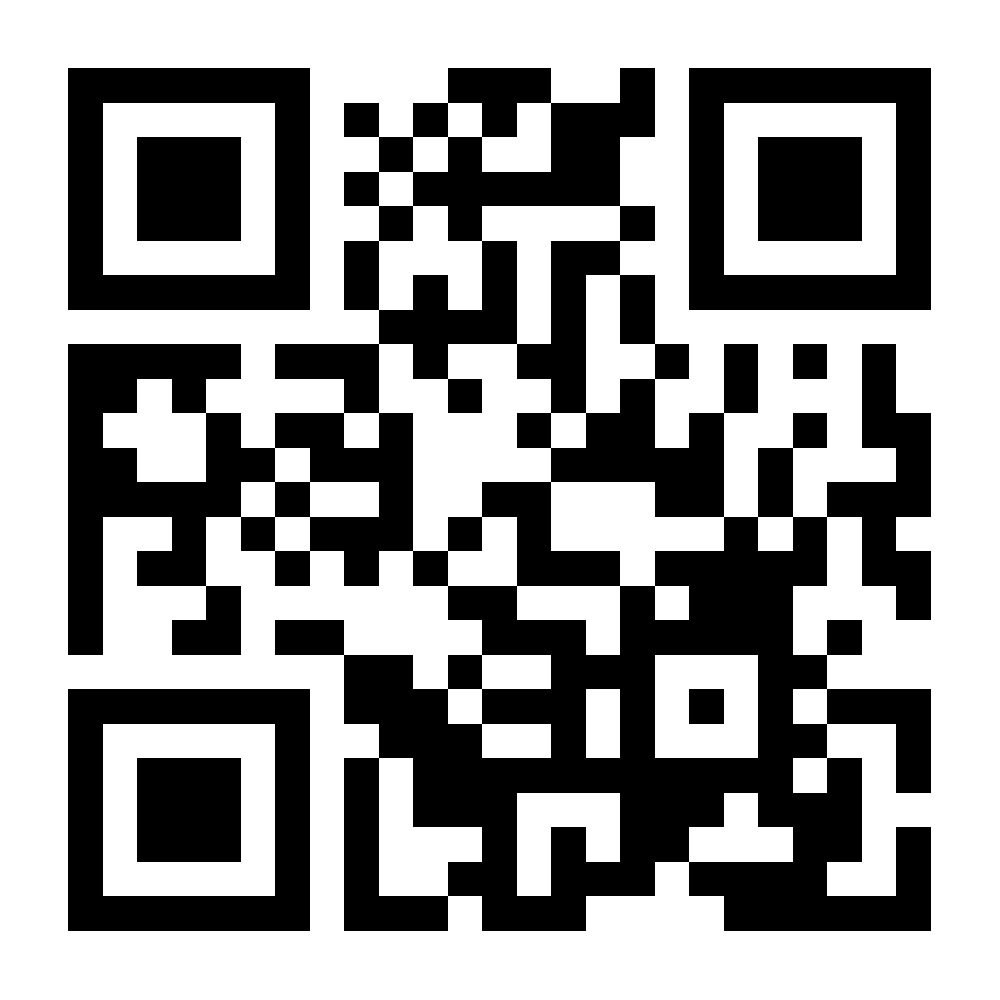
\includegraphics[width=2cm]{Figures Worksheets/qrcode.png}
\newpage
\kariert{Nutzen Sie diese Seite für Notizen}{16}{23}


            
\end{document}